\section{Results} \label{sec:conclusions}
We produce simulated events until we find at least $100$ with sufficiently small localizations that further analysis is practical. This cutoff is arbitrary, for all results reported we used a maximum volume of $0.5\times 10^{9}$\si{Mpc^3}. We also observed values which had anolously small localization volumes so we also constrained all simulated events to have a localization volume larger than $0.5\times 10^{7}$\si{Mpc^3}. We found that a total of (TODO: insert number) observations were needed to produce $100$ desired localizations. Well localized regions corresponded to (TODO: insert percentage) of all generated samples. In all of our tests we injected a known value of $H_0=70$\si{km.s^{-1}.Mpc^{-1}}.

The resulting posterior $p(H_0 | d_{GW}, d_C)$ produced after $100$ observations is shown in figure \ref{fig:posterior} along with the posterior obtained from each observation considered in isolation. In figure \ref{fig:std} we show the standard deviation of the posterior $p(H_0 | d_{GW}, d_C)$ as a function of number of localized events. Some interesting correlations are noticable with events with wider spreads on the posterior tending to center around smaller values of $H_0$. In figure \ref{fig:mean_diff} we show the deviation of the posterior expectation on $H_0$ from the known value as a function of number of well localized events. We can see that our posterior produces an underestimate of $H_0$. This suggests that there are as yet unidentified systematic effects that need to be taken into account. 

\begin{figure}
    \centering
    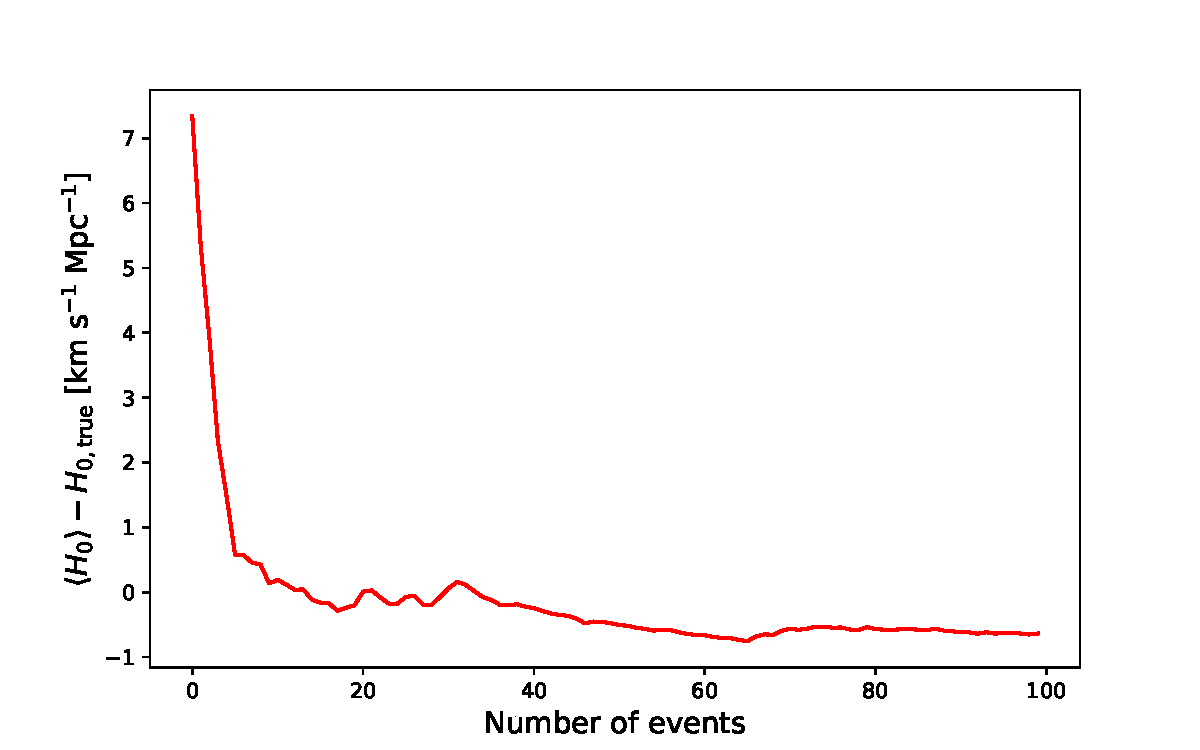
\includegraphics[width=0.95\columnwidth]{figures/diff.pdf}
    \caption{The deviation between the injected known value of $H_0$ and our expectation value based on $p(H_0 | d_{GW}, d_C)$.}
    \label{fig:mean_diff}
\end{figure}

\begin{figure}
    \centering
    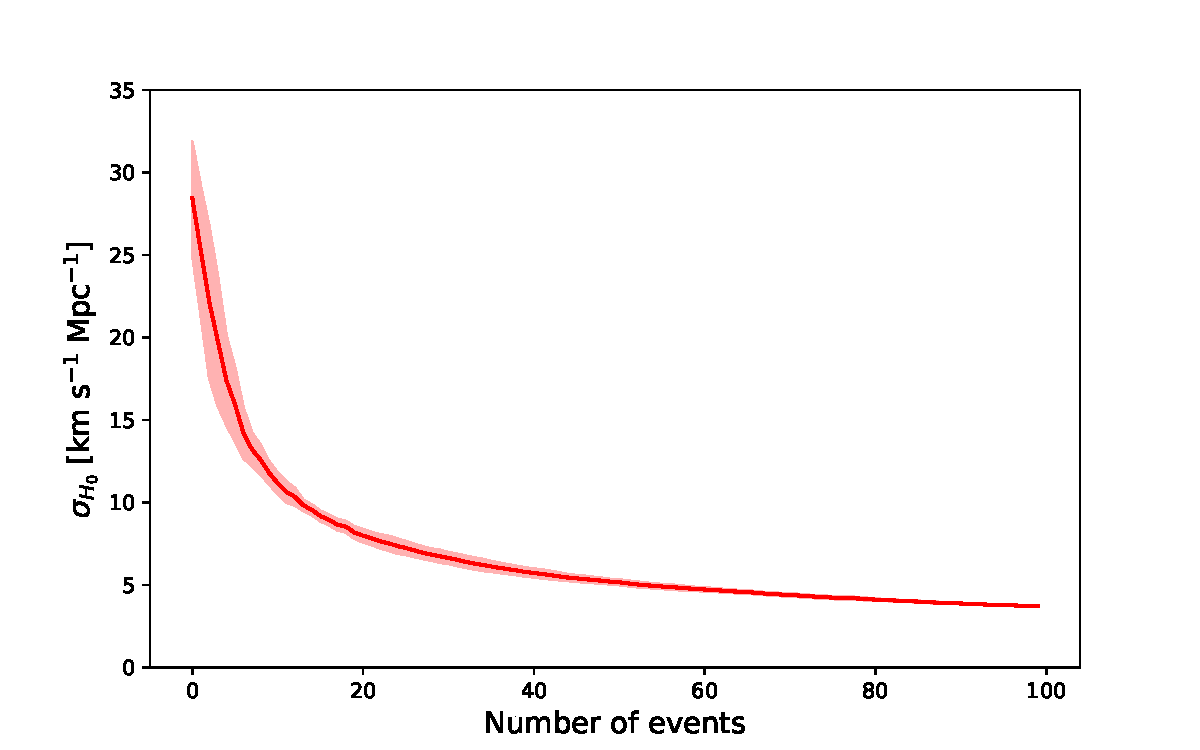
\includegraphics[width=0.95\columnwidth]{figures/std.pdf}
    \caption{The standard deviation obtained from the posterior $p(H_0 | d_{GW}, d_C)$.}
    \label{fig:std}
\end{figure}

\begin{figure}
    \centering
    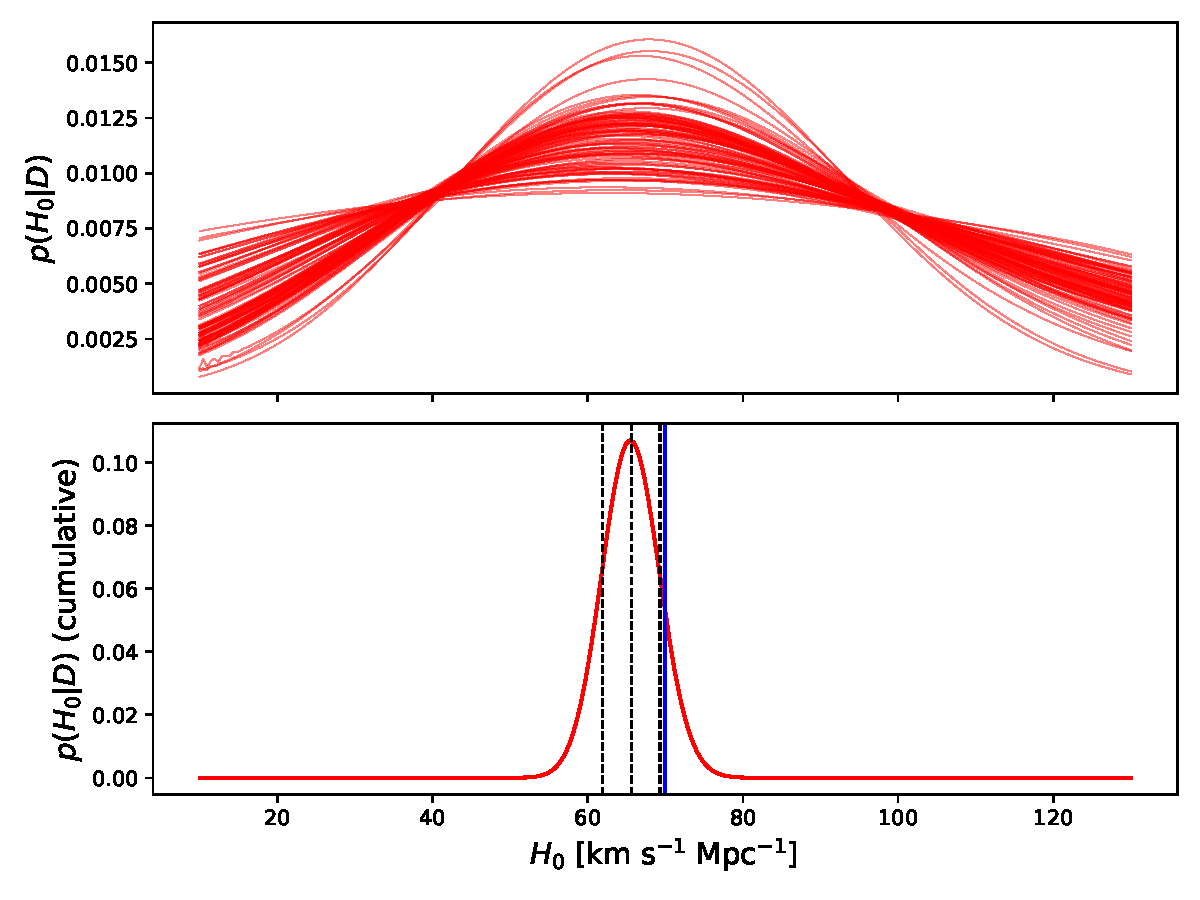
\includegraphics[width=0.95\columnwidth]{figures/posterior.pdf}
    \caption{Upper: Posteriors produced from individual events. The bias of posteriors with poorer localization is noticable, and is probably contributing to the underestimate of $H_0$ that we note. Lower: The posterior $p(H_0 | d_{GW}, d_C)$ produced after $100$ samples. The $68\%$ Confidence interval is shown by the dashed lines. The true injected value is shown in blue.}
    \label{fig:posterior}
\end{figure}
